\section{Introduction}
\IEEEPARstart{P}{roduction-line} integration for an industrial agent couples online data acquisition with governed control. The agent acquires process observations and production context, relates them to an objective, and proposes a typed setpoint or recipe adjustment. The runtime resolves the relevant line, process variable, and control signal before applying authority and limits. For example, a cast-film line-speed setpoint may affect measured film thickness, but the control and acquisition nodes remain distinct even when both use Message Queuing Telemetry Transport (MQTT). Acquired observations, command acceptance, device readback, and later process measurements are separate evidence. Fig.~\ref{fig:control-path} illustrates this distinction.

Research on industrial agents includes service supervision and skill-based manufacturing \cite{biskupovic2025supervision,koehle2026llmdriven}. Other studies examine semantic grounding, approval, and verification for plant-facing operations, including programmable logic controller (PLC) interfaces \cite{graul2026aas,schall2026safe}. Fault-recovery planning is another area of study \cite{vyas2026detection}. Building on these studies, we examine how a runtime can connect an agent's online acquisition and analysis to a controlled operation across task-mediated and direct entry paths. This paper examines that boundary without claiming a new control law or agent-reasoning algorithm.

We enforce five invariants: observations inform an agent proposal but do not grant write authority; acquisition and control mappings are direction-specific; an approved control intent is revalidated; command receipts, readbacks, and later process observations remain separate; and task-mediated and direct calls converge on one guarded boundary. A scene binds line, product, recipe, and run to mappings, drivers, objectives, and limits. Direct API and fixture tests assess selected paths; a complete correlated agent-to-device trace would require retained harness, acquisition, driver, readback, and observation records.

The contributions are:
\begin{enumerate}
  \item A production-scene model linking context, direction-specific acquisition/control mappings, registered drivers, objectives, and limits for agent-facing operations. (Section~III.)
  \item An agent-to-operation boundary in which registered harnesses acquire observations and submit control intents, while task-mediated and direct calls use a shared dispatcher and applicable route-specific approval, revalidation, and write guards. (Sections~III--V.)
  \item An evidence-bounded evaluation of acquisition/control mappings and governance responses, supplemented by an exploratory simulator comparison and language-model-driven episodes. (Section~VI.)
\end{enumerate}

\begin{figure}[!b]
\centering
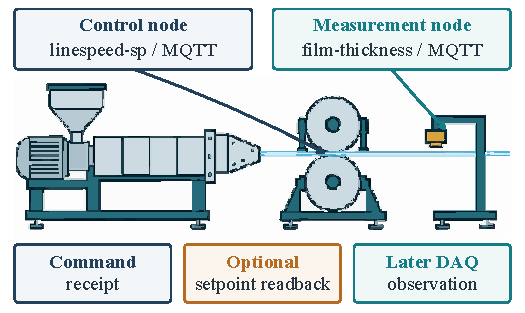
\includegraphics[width=0.98\columnwidth]{resources/fig1-vectorized-20261109.pdf}
\caption{Illustrative configured cast-film example: an agent acquires film-thickness data and may propose a line-speed adjustment, but the line-speed control node and film-thickness acquisition node remain distinct even though both use MQTT. Command acceptance or optional setpoint readback is distinct from the later process observation.}
\label{fig:control-path}
\end{figure}


